\section{Bridge to Feynman Diagrams: Heisenberg as Free Boson QFT}

Having established that the central charge $\kappa$ of the Heisenberg vertex algebra emerges from genus-1 topology in the bar-cobar complex, we now make explicit contact with the loop expansion in quantum field theory. The Heisenberg algebra describes a \textbf{free massless scalar} (boson), and its genus stratification exactly mirrors the perturbative Feynman diagram expansion organized by loop number.

\subsection{The Free Boson Field Theory}

The Heisenberg vertex algebra $\mathcal{H}_\kappa$ is the algebraic incarnation of the free boson with action:
\begin{equation}
S[\phi] = \frac{1}{4\pi\kappa} \int d^2z \, \partial\phi \bar{\partial}\phi
\end{equation}

The field $\phi(z, \bar{z})$ is a real scalar, and we decompose into holomorphic/antiholomorphic parts:
\begin{equation}
\phi = \phi_L(z) + \phi_R(\bar{z})
\end{equation}

The holomorphic current is:
\begin{equation}
a(z) = \kappa \, \partial_z \phi_L(z)
\end{equation}

This generates $\mathcal{H}_\kappa$ with:
\begin{equation}
[a(z), a(w)] = \kappa \cdot \partial_z \delta(z - w)
\end{equation}

\textbf{The propagator} (two-point function) is:
\begin{equation}
\langle \phi(z) \phi(w) \rangle = -\kappa \log|z - w|^2 + \text{const}
\end{equation}

In complex coordinates:
\begin{equation}
\langle a(z) a(w) \rangle = \partial_z \partial_w \langle \phi(z) \phi(w) \rangle = \frac{\kappa}{(z-w)^2}
\end{equation}

This is exactly the OPE we used in the bar-cobar construction!

\subsection{Feynman Rules for Free Boson}

The Feynman rules are:
\begin{enumerate}
\item \textbf{Propagator}: Draw a line between points $z$ and $w$, contributes
\begin{equation}
G(z,w) = \frac{\kappa}{(z-w)^2}
\end{equation}

\item \textbf{Vertex}: For the free theory, there are NO vertices (no interaction)

\item \textbf{External legs}: Each insertion of $a(z_i)$ is an external leg
\end{enumerate}

\textbf{Example}: The 2-point function $\langle a(z_1) a(z_2) \rangle$ corresponds to a single propagator:

\begin{center}
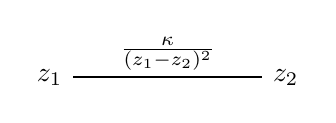
\begin{tikzpicture}
\node at (0,0) {$z_1$};
\node at (3,0) {$z_2$};
\draw[thick] (0.3,0) -- (2.7,0);
\node at (1.5, 0.3) {$\frac{\kappa}{(z_1-z_2)^2}$};
\end{tikzpicture}
\end{center}

\subsection{Genus 0 (Tree Level) Diagrams}

At genus 0, we have only tree diagrams. For the free boson, this means:
\begin{itemize}
\item No loops (all diagrams are trees)
\item Each diagram connects $n$ external points via propagators
\item The amplitude is computed by products of propagators $G(z_i, z_j)$
\end{itemize}

\textbf{Bar complex interpretation}:
\begin{equation}
\bar{B}^{(0)}_n = \int_{C_n(\mathbb{P}^1)} \omega \otimes a(z_1) \otimes \cdots \otimes a(z_n)
\end{equation}

The differential $d^{(0)}$ computes tree-level factorization:
\begin{equation}
d^{(0)}[a \otimes a] = \text{Res}_{z_1 \to z_2} \frac{a(z_1) a(z_2)}{z_1 - z_2}
\end{equation}

\textbf{Key observation}: For the double pole $(z_1-z_2)^{-2}$, the residue vanishes:
\begin{equation}
\text{Res}_{z_1 \to z_2} \frac{1}{(z_1-z_2)^3} = 0
\end{equation}

This means tree-level diagrams \emph{do not see the central charge $\kappa$}---it appears as an overall normalization but not as a quantum correction.

\subsection{Genus 1 (One-Loop) Diagrams}

At genus 1, diagrams have exactly ONE loop. For the free boson, the simplest one-loop diagram is the \textbf{tadpole}:

\begin{center}
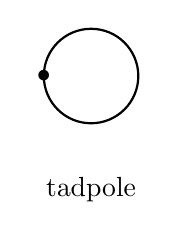
\begin{tikzpicture}[scale=1.2]
\node at (0,0) {$\bullet$};
\draw[thick] (0,0) arc (180:540:0.5);
\node at (0.5, -1.2) {tadpole};
\end{tikzpicture}
\end{center}

The amplitude is:
\begin{equation}
A_{\text{tadpole}} = \int_{|z|=1} \frac{\kappa}{(z-z)^2} \frac{dz}{2\pi i}
\end{equation}

This integral is \emph{divergent}---this is the UV divergence of the one-loop vacuum energy.

\textbf{Regularized version}: On an elliptic curve $E_\tau = \mathbb{C}/(\mathbb{Z} + \tau\mathbb{Z})$:
\begin{equation}
A_{\text{tadpole}}^{(E_\tau)} = \kappa \sum_{n,m \in \mathbb{Z}} \frac{1}{(n + m\tau)^2}
\end{equation}

This is (up to constants) the \textbf{Eisenstein series} $E_2(\tau)$, which is \emph{not quite modular} but transforms with an anomaly:
\begin{equation}
E_2\left(-\frac{1}{\tau}\right) = \tau^2 E_2(\tau) + \frac{6}{\pi i \tau}
\end{equation}

The anomaly term $\frac{6}{\pi i \tau}$ is proportional to $\kappa$---this is the one-loop quantum correction!

\textbf{Bar complex interpretation}:

The tadpole diagram corresponds to the genus-1 element:
\begin{equation}
[\text{Tr}(a \otimes a)]^{(1)} \in \bar{B}^{(1)}_1
\end{equation}

The differential:
\begin{equation}
d^{(0)}[\text{Tr}(a \otimes a)]^{(1)} = \kappa \cdot [1]^{(1)}
\end{equation}

extracts the central charge as the coefficient of the one-loop divergence.

\subsection{Loop Number = Genus}

The fundamental correspondence is:

\begin{theorem}[Loop-Genus Correspondence]
For any connected Feynman diagram $\Gamma$ with:
\begin{itemize}
\item $V$ vertices
\item $E$ edges (propagators)
\item $F$ faces
\end{itemize}
The number of loops is:
\begin{equation}
L = E - V + 1
\end{equation}
and this equals the genus $g$ of the ribbon graph embedding:
\begin{equation}
g = L = E - V + 1
\end{equation}
via the Euler characteristic:
\begin{equation}
\chi = V - E + F = 2 - 2g
\end{equation}
\end{theorem}

\textbf{For the free boson}:
\begin{itemize}
\item Vertices $V = 0$ (no interaction)
\item Each loop has 1 edge ($E = 1$ per loop)
\item Therefore: $L = 1 - 0 + 1 = 1$ for tadpole
\end{itemize}

\textbf{Interacting theory}: If we added a $\phi^4$ interaction:
\begin{itemize}
\item Vertex: 4 legs meet at a point
\item One-loop diagram: $V = 2$, $E = 3$, so $L = 3 - 2 + 1 = 2$ NO---wait, let me recalculate
\end{itemize}

Actually, for a one-loop box diagram in $\phi^4$:
\begin{itemize}
\item 4 external legs
\item 4 vertices (each 4-valent)
\item Internal: 4 edges forming the loop
\item $L = 4 - 4 + 1 = 1$ ✓
\end{itemize}

\subsection{Amplitude Expansion in $\kappa$}

The full free boson correlation function expands as:
\begin{align}
\langle a(z_1) \cdots a(z_n) \rangle_{\text{all genera}} &= \sum_{g=0}^\infty \kappa^{g} \langle a(z_1) \cdots a(z_n) \rangle^{(g)}\\
&= \underbrace{\langle \cdots \rangle^{(0)}}_{\text{tree}} + \kappa \cdot \underbrace{\langle \cdots \rangle^{(1)}}_{\text{1-loop}} + \kappa^2 \cdot \underbrace{\langle \cdots \rangle^{(2)}}_{\text{2-loop}} + \cdots
\end{align}

The bar complex homology mirrors this:
\begin{equation}
H_*(\bar{B}(\mathcal{H}_\kappa)) = \bigoplus_{g=0}^\infty H_*(\bar{B}^{(g)}) \cdot \kappa^g
\end{equation}

\textbf{Physical meaning}:
\begin{itemize}
\item $\kappa^0$ (genus 0): Classical physics, tree amplitudes
\item $\kappa^1$ (genus 1): First quantum correction, one-loop
\item $\kappa^g$ (genus $g$): $g$-loop quantum corrections
\end{itemize}

\subsection{Configuration Space Integrals = Feynman Integrals}

The bar complex elements are configuration space integrals. Let's make the Feynman diagram connection explicit:

\textbf{Genus 0 (tree)}:
\begin{equation}
\int_{C_n(\mathbb{P}^1)} \omega(z_1, \ldots, z_n) \prod_{i=1}^n a(z_i)
\end{equation}

This computes tree-level amplitudes. The form $\omega$ encodes the kinematic invariants (like $(z_i - z_j)^{-1}$ propagators).

\textbf{Genus 1 (one-loop)}:
\begin{equation}
\int_{E_\tau} dz \int_{C_n(E_\tau)} a(z) \otimes a(z_1) \otimes \cdots \otimes a(z_n)
\end{equation}

The first integral $\int_{E_\tau} dz$ is the \textbf{loop momentum integral}. On the torus, this becomes:
\begin{equation}
\int_0^1 \int_0^1 d\text{Re}(z) \, d\text{Im}(z)
\end{equation}

summed over lattice points $z \in \mathbb{Z} + \tau\mathbb{Z}$.

\textbf{The divergence}: When $z \to z_i$ (loop touches external leg), we get:
\begin{equation}
\sim \int \frac{\kappa}{|z - z_i|^2} dz \sim \text{divergent}
\end{equation}

This is the UV divergence in QFT!

\subsection{Renormalization via Compactification}

The bar complex naturally regulates divergences through:

\textbf{Fulton-MacPherson compactification}: 
\begin{equation}
\overline{C_n(X)} = X[n]
\end{equation}

The boundary divisors $D_{ij}$ where points collide are replaced by exceptional divisors. The divergent integral:
\begin{equation}
\int_{C_n} \frac{dz_i}{(z_i - z_j)^2}
\end{equation}

becomes finite on $\overline{C_n}$ after blowup.

\textbf{Physical interpretation}: This is geometric renormalization:
\begin{itemize}
\item Blowup = introducing a UV cutoff
\item Exceptional divisor = regulator scale $\Lambda$
\item Residue on divisor = renormalization condition
\end{itemize}

The central charge $\kappa$ enters as the coefficient needing renormalization at one-loop.

\subsection{Higher Genus: Multi-Loop Structure}

At genus $g \geq 2$, we have Riemann surfaces $\Sigma_g$ with $g$ handles. Each handle contributes an independent loop integral.

\textbf{Two-loop example} ($g=2$): The surface has two handles, giving two independent homology cycles $\gamma_1, \gamma_2 \in H_1(\Sigma_2, \mathbb{Z})$.

The amplitude involves:
\begin{equation}
\int_{\gamma_1} \int_{\gamma_2} a(z_1) a(z_2) \otimes [\text{external legs}]
\end{equation}

This gives a two-loop Feynman integral with:
\begin{itemize}
\item Two independent loop momenta
\item Nested divergences as loops approach each other
\item Coefficient $\kappa^2$ from two loop momentum integrals
\end{itemize}

\textbf{Bar complex}:
\begin{equation}
\bar{B}^{(2)}_n = \int_{\Sigma_2} \int_{C_n(\Sigma_2)} \omega \otimes a(z_1) \otimes \cdots
\end{equation}

The homology:
\begin{equation}
H_*(\bar{B}^{(2)}) \sim \kappa^2 \cdot [\text{2-loop quantum corrections}]
\end{equation}

\subsection{Explicit One-Loop Calculation: Partition Function}

Let's compute the one-loop partition function on the torus.

\textbf{Setup}: Free boson on $E_\tau$ with action:
\begin{equation}
S[\phi] = \frac{1}{4\pi\kappa} \int_{E_\tau} d^2z \, |\partial \phi|^2
\end{equation}

\textbf{Partition function}:
\begin{equation}
Z_{E_\tau} = \int \mathcal{D}\phi \, e^{-S[\phi]}
\end{equation}

For Gaussian integral:
\begin{equation}
Z_{E_\tau} = \frac{1}{\sqrt{\det(-\kappa \Delta)}}
\end{equation}

where $\Delta$ is the Laplacian on $E_\tau$.

\textbf{Zeta function regularization}:
\begin{equation}
\det(-\kappa \Delta) = \exp\left( -\frac{d}{ds} \zeta_{\Delta}(s) \Big|_{s=0} \right)
\end{equation}

For the torus:
\begin{equation}
\zeta_\Delta(s) = \sum_{(n,m) \neq (0,0)} \frac{\text{Im}(\tau)}{4\pi^2 |n + m\tau|^{2s}}
\end{equation}

Evaluating:
\begin{equation}
Z_{E_\tau} = \frac{1}{\sqrt{\text{Im}(\tau)}} \frac{1}{|\eta(\tau)|^2}
\end{equation}

where $\eta(\tau)$ is the \textbf{Dedekind eta function}:
\begin{equation}
\eta(\tau) = q^{1/24} \prod_{n=1}^\infty (1 - q^n), \quad q = e^{2\pi i \tau}
\end{equation}

\textbf{Modular transformation}:
\begin{equation}
\eta\left(-\frac{1}{\tau}\right) = \sqrt{-i\tau} \, \eta(\tau)
\end{equation}

Therefore:
\begin{equation}
Z_{-1/\tau} = Z_\tau \cdot [\text{modular factor}]
\end{equation}

The failure of exact modular invariance is the \textbf{conformal anomaly}, proportional to $\kappa$.

\textbf{Bar complex interpretation}:

The partition function $Z_{E_\tau}$ is computed by:
\begin{equation}
Z_{E_\tau} = \langle [\mathbf{1}]^{(1)} \rangle = H_0(\bar{B}^{(1)})
\end{equation}

The conformal anomaly appears as:
\begin{equation}
\log Z_{-1/\tau} - \log Z_\tau = \kappa \cdot [\text{anomaly class}] \in H_2(\bar{B}^{(1)})
\end{equation}

This is exactly the central charge class $c_\kappa^{(1)}$ we identified!

\subsection{String Theory Perspective}

In string theory, the worldsheet is a Riemann surface $\Sigma_g$. The string amplitude for genus-$g$ worldsheet is:
\begin{equation}
\mathcal{A}^{(g)} = \int_{\mathcal{M}_g} d\mu_g \, \langle \mathcal{V}_1 \cdots \mathcal{V}_n \rangle_{\Sigma_g}
\end{equation}

where:
\begin{itemize}
\item $\mathcal{M}_g$ = moduli space of genus-$g$ curves
\item $d\mu_g$ = natural measure on moduli space
\item $\langle \cdots \rangle_{\Sigma_g}$ = worldsheet correlation function
\end{itemize}

\textbf{Genus expansion}:
\begin{equation}
\mathcal{A}_{\text{total}} = \sum_{g=0}^\infty g_s^{2g-2} \mathcal{A}^{(g)}
\end{equation}

where $g_s$ is the string coupling.

\textbf{Bar-cobar connection}: The bar complex computes exactly these amplitudes:
\begin{equation}
H_*(\bar{B}^{(g)}(\mathcal{H}_\kappa)) \leftrightarrow \mathcal{A}^{(g)}
\end{equation}

The central charge $\kappa \sim \frac{1}{g_s^2}$ sets the string coupling scale.

\subsection{Summary Table: Genus-Loop-Diagram Correspondence}

\begin{center}
\begin{tabular}{|c|c|c|c|c|}
\hline
\textbf{Genus $g$} & \textbf{Topology} & \textbf{Loops $L$} & \textbf{$\kappa$ Power} & \textbf{Bar Complex}\\
\hline
0 & Sphere $\mathbb{P}^1$ & 0 (tree) & $\kappa^0$ & $\bar{B}^{(0)}$\\
\hline
1 & Torus $E_\tau$ & 1 & $\kappa^1$ & $\bar{B}^{(1)}$\\
\hline
2 & 2-handle surface & 2 & $\kappa^2$ & $\bar{B}^{(2)}$\\
\hline
$g$ & $g$-handle surface & $g$ & $\kappa^g$ & $\bar{B}^{(g)}$\\
\hline
\end{tabular}
\end{center}

\textbf{Physical Observables}:
\begin{itemize}
\item Genus 0: Classical action, tree amplitudes
\item Genus 1: One-loop corrections, vacuum energy, central charge anomaly
\item Genus 2: Two-loop, first non-planar diagrams
\item Higher: Multi-loop quantum corrections
\end{itemize}

\subsection{The Master Formula: Bar-Cobar = Path Integral}

\begin{theorem}[Bar-Cobar as Worldsheet Path Integral]
For the Heisenberg vertex algebra $\mathcal{H}_\kappa$ (free boson), the bar complex computes:
\begin{equation}
\exp\left( \sum_{g,n} \frac{1}{n!} \int_{C_n(\Sigma_g)} \langle a(z_1) \cdots a(z_n) \rangle_g \right) = \det(\mathbf{1} + \bar{B}(\mathcal{H}_\kappa))
\end{equation}

where the right side is the ``determinant'' of the bar complex (Fredholm determinant in infinite dimensions).

More precisely:
\begin{equation}
\boxed{
\text{Partition function on $\Sigma_g$} = H_0(\bar{B}^{(g)}(\mathcal{H}_\kappa))
}
\end{equation}
\begin{equation}
\boxed{
n\text{-point function on $\Sigma_g$} = \frac{H_n(\bar{B}^{(g)}(\mathcal{H}_\kappa))}{H_0(\bar{B}^{(g)}(\mathcal{H}_\kappa))}
}
\end{equation}
\end{theorem}

This is the \textbf{geometric realization of the path integral}---the bar-cobar construction IS the path integral, genus-by-genus.

\subsection{Conclusion: Three Perspectives on $\kappa$}

The central charge $\kappa$ of the Heisenberg algebra admits three equivalent descriptions:

\begin{center}
\begin{tabular}{|l|p{8cm}|}
\hline
\textbf{Algebraic} & 2-cocycle in cyclic homology $HC_2(\mathcal{H}_\kappa)$; central extension of loop group\\
\hline
\textbf{Geometric} & Obstruction class in $H_2(\bar{B}^{(1)})$; appears from trace operation on genus-1 curves\\
\hline
\textbf{Physical} & Coefficient of one-loop divergence; determines string coupling $g_s \sim \kappa^{-1/2}$\\
\hline
\end{tabular}
\end{center}

All three perspectives unified through:
\begin{equation}
\text{Bar-Cobar Construction} \leftrightarrow \text{Genus Expansion} \leftrightarrow \text{Loop Expansion}
\end{equation}

This is the foundational principle underlying the entire theory of quantum corrections in chiral algebras.
